% Provenance (never printed): old seconde/premiere S material on the
% atmosphere (water vapour, saturation, cloud formation, the vertical motion
% of air) and enseignement scientifique premiere (water cycle); see
% sources/book2/PROVENANCE.md. Every saturation value, lapse rate,
% condensation level and the lee-wind example are computed in
% figdata/grade-10/clouds.py from the IAPWS saturation curves; the soundings
% are invented examples, said so in the text.
\chapter{Mengapa Awan Terbentuk}\label{ch:g10:why-clouds-form}

Di sebuah teras pada musim panas, segelas air es berdiri di atas meja. Dalam
semenit, sisi luarnya tertutup titik-titik air yang kecil, dan genangan air
melebar di kakinya. Air itu tidak merembes menembus gelas: air itu keluar dari
udara, yang mendingin di tempat udara itu menyentuh gelas yang dingin.
Beberapa jam kemudian, berkilometer-kilometer di atas dataran, hal yang sama
terjadi dalam skala besar: gelembung-gelembung udara hangat naik, mendingin,
dan pada ketinggian tertentu air yang dibawanya muncul sebagai gumpalan awan
putih berdasar datar yang disebut kumulus. Bab ini menjelaskan seberapa banyak
uap air yang dapat ditampung udara, mengapa udara yang naik mendingin, pada
ketinggian berapa awan terbentuk, mengapa pada hari tertentu awan tetap datar
sedangkan pada hari lain menjulang menjadi badai guntur, dan bagaimana
titik-titik awan yang mungil berubah menjadi hujan dan salju.

\begin{omfigure}
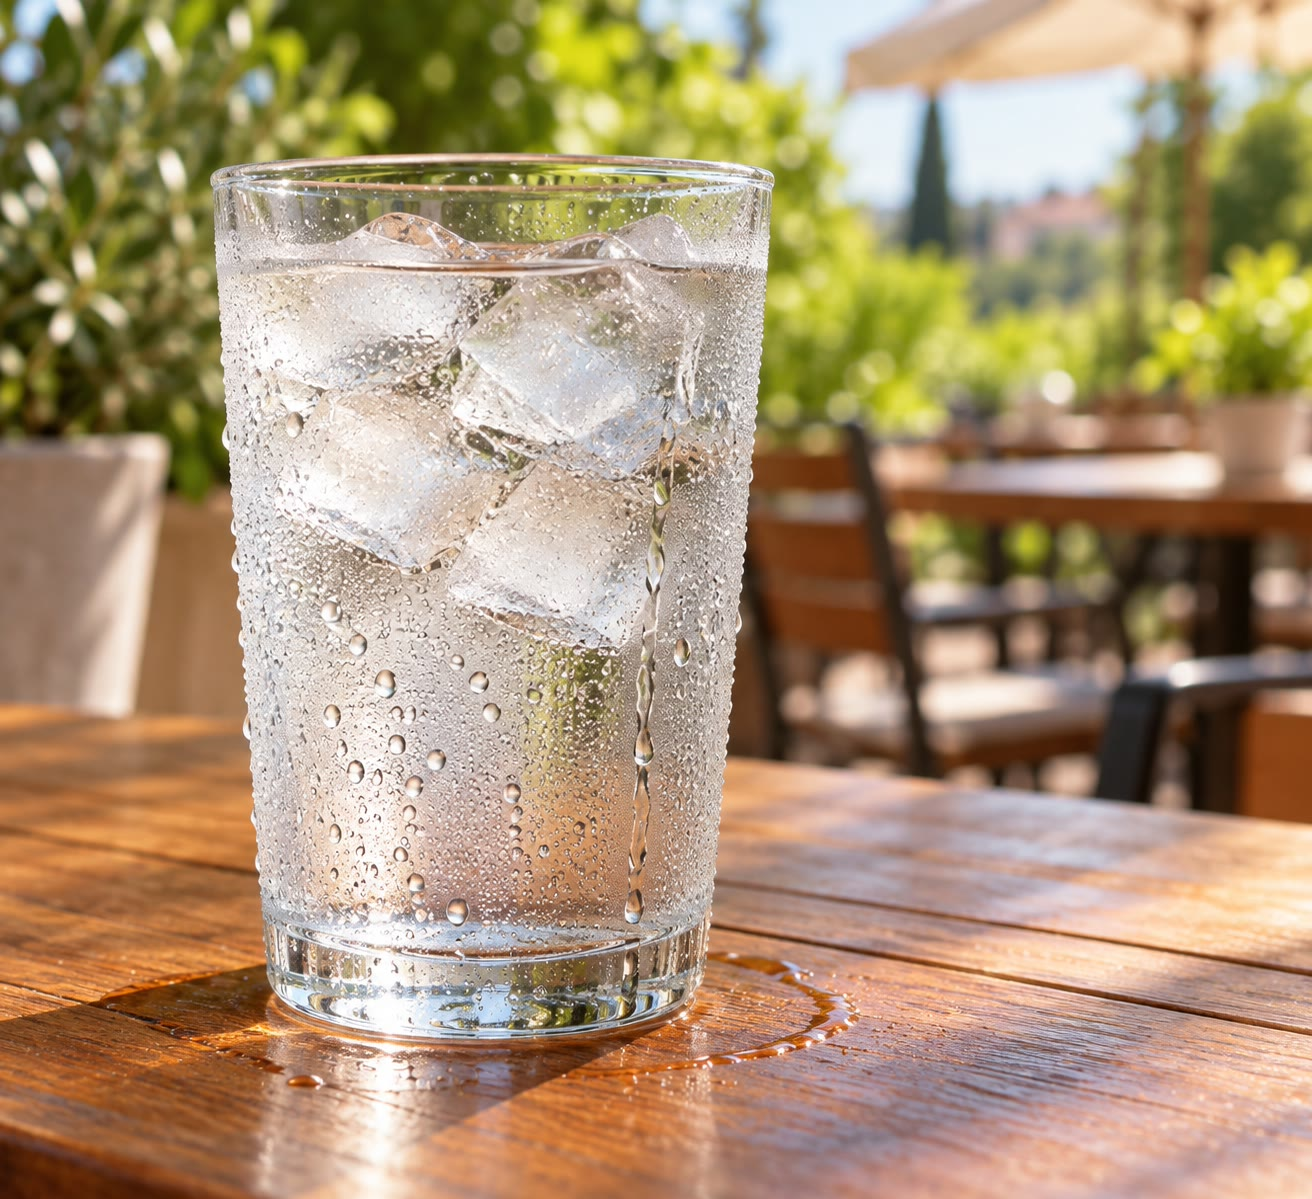
\includegraphics[width=0.5\linewidth]{images/book2/ai/g10-cold-glass.jpg}

{\small Segelas air es di teras pada musim panas: titik-titik air terbentuk di
sisi luarnya, tempat udara yang menyentuh gelas itu mendingin.}
\end{omfigure}

\begin{recall}
Awan terdiri atas titik-titik air atau kristal-kristal es yang sangat kecil;
awan dikelompokkan menurut bentuk dan ketinggiannya, dan awan menghasilkan
hujan, salju, dan hujan es, yang diukur dengan penakar hujan (Buku 1, kelas
4). Suhu udara turun terhadap ketinggian di lapisan terbawah atmosfer,
rata-rata sekitar \qty{6.5}{\degreeCelsius} per kilometer; inilah laju
penurunan suhu lingkungan, dan front memisahkan massa-massa udara yang suhunya
berbeda (Buku 1, kelas 8). Tekanan turun terhadap ketinggian (buku-buku
fisika). Air menguap dan mengembun, dan penguapan menyerap \omterm{def:g10:earth-energy-budget:latent-heat}{kalor laten} yang
dilepaskan kembali oleh pengembunan (buku-buku fisika dan
\cref{ch:g10:earth-energy-budget}).
\end{recall}
% ledger: nasa:grc-atmosphere

\section{Uap air dan kejenuhan}

Udara selalu mengandung sejumlah uap air, yaitu gas yang tidak terlihat.
Seberapa banyak uap air yang dapat dikandungnya terutama bergantung pada
suhunya.

\begin{definition}[Kejenuhan; kelembapan relatif]\label{def:g10:why-clouds-form:humidity}
Udara disebut \emph{jenuh}\index{kejenuhan} bila mengandung massa uap air
terbesar yang dapat ditampungnya pada suhunya, yaitu \emph{kandungan
jenuhnya}; uap tambahan apa pun mengembun menjadi titik-titik air. Yang
disebut \emph{kelembapan relatif}\index{kelembapan relatif} udara adalah
kandungan uap airnya dibagi kandungan jenuhnya pada suhu dan tekanan yang
sama, dinyatakan dalam persen.
\end{definition}

Kandungan air dalam udara di sini diukur dalam gram uap per kilogram udara
kering (\unit{g/kg}): parsel udara yang naik atau turun tanpa memperoleh atau
kehilangan air kandungannya tetap sama, meskipun parsel itu memuai.

\begin{omfigure}
\begin{tikzpicture}
\begin{axis}[omrecord, width=0.88\linewidth, height=6.2cm, xmin=-10, xmax=40,
  ymin=0, ymax=50, xlabel={suhu (\unit{\degreeCelsius})},
  ylabel={kandungan jenuh (\unit{g/kg})}, xtick={-10,0,...,40},
  tick label style={font=\small}, label style={font=\small}]
\addplot[omDef!85!black, thick] table[x=T_C, y=ws_gkg] {figdata/out/grade-10-clouds-sat.dat};
\addplot[only marks, mark=*, mark size=1.8pt, omThm!85!black] coordinates {(28,11.37)};
\addplot[only marks, mark=o, mark size=1.8pt, omThm!85!black] coordinates {(16,11.37)};
\draw[->, omThm!85!black, thick] (axis cs:27.2,11.37) -- (axis cs:16.9,11.37);
\node[anchor=north, font=\footnotesize, omThm!85!black] at (axis cs:28,10.6) {udara bersuhu \qty{28}{\degreeCelsius}};
\node[anchor=south east, font=\footnotesize, omThm!85!black] at (axis cs:15.5,12.2) {titik embun};
\node[anchor=south east, font=\footnotesize, omDef!85!black, align=right] at (axis cs:31,34) {di atas kurva:\\uap mengembun};
\node[anchor=south west, font=\footnotesize, omDef!85!black] at (axis cs:31,2.5) {tidak jenuh};
\node[anchor=north west, font=\footnotesize, omDef!85!black] at (axis cs:34,31.5) {kejenuhan};
\end{axis}
\end{tikzpicture}

{\small Massa uap air terbesar yang dapat ditampung satu kilogram udara,
terhadap suhu, pada tekanan permukaan laut (di atas air cair; dihitung dari
standar internasional untuk air). Udara bersuhu \qty{28}{\degreeCelsius} yang
mengandung \qty{11.4}{g/kg} (titik) jauh dari \omterm{def:g10:why-clouds-form:humidity}{jenuh}; bila didinginkan tanpa
kehilangan air, udara itu menjadi \omterm{def:g10:why-clouds-form:humidity}{jenuh} pada \qty{16}{\degreeCelsius}
(lingkaran).}
\end{omfigure}
% ledger: iapws:vapour-pressure, ciaaw:abridged-2024, earth:Mmol, const:R (computed in figdata/grade-10/clouds.py)

Kurva itu naik dengan curam: \qty{3.8}{g/kg} pada \qty{0}{\degreeCelsius},
\qty{14.7}{g/kg} pada \qty{20}{\degreeCelsius}, \qty{27.2}{g/kg} pada
\qty{30}{\degreeCelsius}. Setiap pemanasan \qty{10}{\degreeCelsius} hampir
menggandakan air yang dapat ditampung udara. Itulah sebabnya udara tropis
dapat membawa hujan lebat, dan udara musim dingin kutub, sekalipun \omterm{def:g10:why-clouds-form:humidity}{jenuh},
hampir tidak mengandung apa-apa.

\begin{definition}[Titik embun]\label{def:g10:why-clouds-form:dew-point}
Yang disebut \emph{titik embun}\index{titik embun} udara adalah suhu yang
harus dicapai udara itu bila didinginkan, dengan kandungan air dan tekanannya
tetap, agar menjadi \omterm{def:g10:why-clouds-form:humidity}{jenuh}.
\end{definition}

\begin{method}[Kelembapan relatif dan titik embun dari tabel]\label{met:g10:why-clouds-form:table}
\begin{enumerate}
  \item Baca dalam tabel kandungan \omterm{def:g10:why-clouds-form:humidity}{jenuh} pada suhu udara itu.
  \item \omterm{def:g10:why-clouds-form:humidity}{Kelembapan relatif}: bagilah kandungan air udara dengan nilai itu.
  \item \omterm{def:g10:why-clouds-form:dew-point}{Titik embun}: carilah dalam tabel suhu yang kandungan \omterm{def:g10:why-clouds-form:humidity}{jenuhnya} sama
        dengan kandungan air udara.
\end{enumerate}
\end{method}

\begin{example}[Suatu pagi musim panas]\label{ex:g10:why-clouds-form:morning}
% ledger: iapws:vapour-pressure (values computed in figdata/grade-10/clouds.py)
Pada \qty{20}{\degreeCelsius} udara mengandung \qty{11.4}{g/kg}. Kandungan
\omterm{def:g10:why-clouds-form:humidity}{jenuh} pada \qty{20}{\degreeCelsius} adalah \qty{14.7}{g/kg}, jadi \omterm{def:g10:why-clouds-form:humidity}{kelembapan
relatifnya} $11.4/14.7 \approx \qty{78}{\percent}$. Kandungan \omterm{def:g10:why-clouds-form:humidity}{jenuhnya}
\qty{11.4}{g/kg} pada \qty{16}{\degreeCelsius}: itulah \omterm{def:g10:why-clouds-form:dew-point}{titik embunnya}. Pada
sore hari, udara yang sama yang telah menghangat menjadi
\qty{28}{\degreeCelsius} (kandungan \omterm{def:g10:why-clouds-form:humidity}{jenuh} \qty{24.1}{g/kg}) hanya memiliki
\omterm{def:g10:why-clouds-form:humidity}{kelembapan relatif} \qty{47}{\percent} --- dengan jumlah air yang tepat sama.
\end{example}

Gelas pada awal bab lebih dingin daripada \omterm{def:g10:why-clouds-form:dew-point}{titik embun} udara di sekitarnya:
udara yang menyentuhnya didinginkan sampai di bawah \omterm{def:g10:why-clouds-form:dew-point}{titik embunnya} dan
melepaskan air pada gelas. Pada malam yang cerah, rumput dan atap mobil
kehilangan kalor dengan memancarkan inframerah ke langit dan menjadi lebih
dingin daripada udara: embun terbentuk di atasnya, atau embun beku di bawah
\qty{0}{\degreeCelsius}. Bila seluruh lapisan udara di dekat tanah mendingin
sampai \omterm{def:g10:why-clouds-form:dew-point}{titik embunnya}, titik-titik air terbentuk di dalam udara itu sendiri:
itulah kabut.

\begin{omfigure}
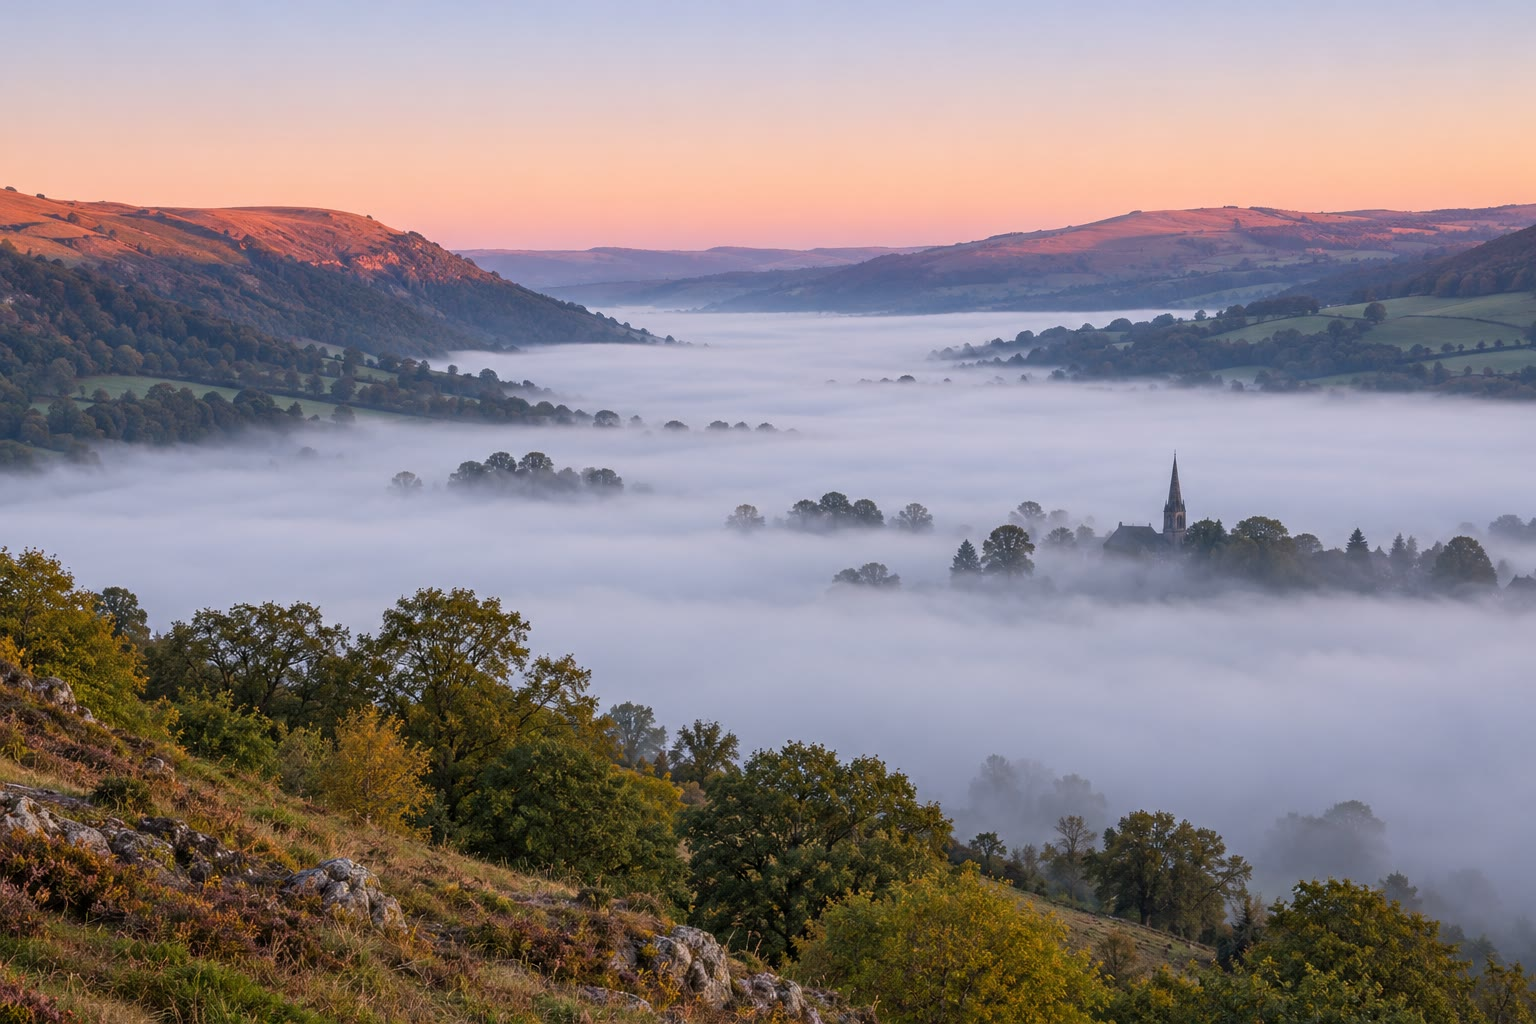
\includegraphics[width=0.75\linewidth]{images/book2/ai/g10-valley-fog.jpg}

{\small Kabut memenuhi sebuah lembah pada waktu fajar. Selama malam yang
cerah, tanah mendingin, udara dingin mengalir turun ke lembah, dan di sana
udara itu mendingin sampai di bawah \omterm{def:g10:why-clouds-form:dew-point}{titik embunnya}.}
\end{omfigure}

\section{Udara yang naik mendingin}

Sebagian besar awan tidak terbentuk karena udara menyentuh sesuatu yang
dingin. Awan terbentuk karena udara naik. Tekanan turun terhadap ketinggian;
parsel udara yang naik memuai dan mendorong udara di sekitarnya, dan energi
untuk usaha ini diambil dari parsel itu sendiri.

\begin{definition}[Pendinginan adiabatik; laju adiabatik kering]\label{def:g10:why-clouds-form:adiabatic}
Yang disebut \emph{pendinginan adiabatik}\index{pendinginan adiabatik} adalah
pendinginan parsel udara yang memuai tanpa bertukar kalor dengan
sekitarnya. Laju pendinginan udara tak \omterm{def:g10:why-clouds-form:humidity}{jenuh} yang naik dengan cara ini
disebut \emph{laju adiabatik kering}\index{laju adiabatik kering}, mendekati
\qty{9.8}{\degreeCelsius} per kilometer kenaikan; udara yang turun menghangat
dengan laju yang sama.
\end{definition}

\begin{proposition}[Laju adiabatik kering]\label{prop:g10:why-clouds-form:dry-rate}
\omterm{def:g10:why-clouds-form:adiabatic}{Laju adiabatik kering} adalah $g/c_p$, dengan $g = \qty{9.81}{m/s^2}$ dan $c_p
\approx \qty{1005}{J.kg^{-1}.K^{-1}}$ adalah energi yang menghangatkan satu
kilogram udara sebesar satu derajat pada tekanan tetap: $9.81/1005 \approx
\qty{0.0098}{\degreeCelsius/m}$, yaitu \qty{9.8}{\degreeCelsius/km}.
(Diterima tanpa bukti: buktinya termasuk buku-buku fisika.)
\end{proposition}
% ledger: const:gn, const:R, earth:Mmol (c_p of dry air computed as (7/2)R/M in figdata/grade-10/clouds.py)

\omterm{def:g10:why-clouds-form:dew-point}{Titik embun} parsel itu juga turun ketika parsel naik, tetapi perlahan:
kandungan airnya tetap sama, sedangkan penurunan tekanan membuat uap sedikit
lebih mudah menjadi \omterm{def:g10:why-clouds-form:humidity}{jenuh}. Perhitungan untuk udara di dekat tanah memberikan
sekitar \qty{1.8}{\degreeCelsius} per kilometer. Karena itu suhu parsel
mendekati \omterm{def:g10:why-clouds-form:dew-point}{titik embunnya} sekitar $9.8 - 1.8 = \qty{8}{\degreeCelsius}$ untuk
setiap kilometer kenaikannya.
% ledger: iapws:vapour-pressure (dew-point rate computed in figdata/grade-10/clouds.py)

\begin{definition}[Aras kondensasi]\label{def:g10:why-clouds-form:condensation-level}
Yang disebut \emph{aras kondensasi}\index{aras kondensasi} parsel udara adalah
ketinggian tempat parsel itu, ketika naik, menjadi \omterm{def:g10:why-clouds-form:humidity}{jenuh}. Di atasnya air
mengembun: aras kondensasi adalah dasar datar awan-awan yang dibentuk oleh
udara yang naik.
\end{definition}

\begin{proposition}[Ketinggian aras kondensasi]\label{prop:g10:why-clouds-form:lcl}
Udara yang naik dari tanah dengan suhu $T$ dan \omterm{def:g10:why-clouds-form:dew-point}{titik embun} $T_d$
(dalam \unit{\degreeCelsius}) menjadi \omterm{def:g10:why-clouds-form:humidity}{jenuh} pada ketinggian sekitar
\[
  z = \frac{T - T_d}{8}\ \text{km} = \qty{125}{m} \times (T - T_d).
\]
\end{proposition}

\begin{proof}
Pada ketinggian $z$ (dalam km) suhu parsel adalah $T - 9.8\,z$ dan \omterm{def:g10:why-clouds-form:dew-point}{titik
embunnya} $T_d - 1.8\,z$. Parsel itu \omterm{def:g10:why-clouds-form:humidity}{jenuh} bila keduanya sama:
$T - 9.8\,z = T_d - 1.8\,z$, jadi $8\,z = T - T_d$ dan $z = (T - T_d)/8$ km.
Seperdelapan kilometer adalah \qty{125}{m}.
\end{proof}

\begin{example}[Kumulus sore hari]\label{ex:g10:why-clouds-form:base}
% ledger: iapws:vapour-pressure (exact ascent computed in figdata/grade-10/clouds.py: 1.51 km)
Pada sore hari dalam \cref{ex:g10:why-clouds-form:morning}, udara di tanah
bersuhu \qty{28}{\degreeCelsius} dengan \omterm{def:g10:why-clouds-form:dew-point}{titik embun}
\qty{16}{\degreeCelsius}. Gelembung-gelembung yang naik menjadi \omterm{def:g10:why-clouds-form:humidity}{jenuh} pada
$125 \times 12 = \qty{1500}{m}$: dasar datar kumulus berada sekitar
\qty{1.5}{km} di atas tanah. Pada pagi hari, pada \qty{20}{\degreeCelsius},
udara yang sama sudah mengembun pada ketinggian $125 \times 4 = \qty{500}{m}$
saja: dasar awan naik sepanjang hari seiring menghangatnya tanah.
\end{example}

\section{Udara stabil dan udara tidak stabil}

Apakah parsel yang naik terus naik bergantung pada udara di sekitarnya. Parsel
yang lebih hangat daripada sekitarnya lebih ringan daripada udara yang
didesaknya dan naik, seperti balon udara panas; parsel yang lebih dingin
daripada sekitarnya turun kembali.

\begin{definition}[Udara stabil; udara tidak stabil]\label{def:g10:why-clouds-form:stability}
Udara disebut \emph{stabil}\index{udara stabil} bila parsel yang didorong ke
atas menjadi lebih dingin daripada udara di sekitarnya, sehingga turun kembali
ke tempat asalnya. Udara disebut \emph{tidak stabil}\index{udara tidak stabil}
bila parsel itu menjadi lebih hangat daripada udara di sekitarnya dan terus
naik dengan sendirinya.
\end{definition}

Parsel yang naik mendingin dengan \omterm{def:g10:why-clouds-form:adiabatic}{laju adiabatik kering},
\qty{9.8}{\degreeCelsius} per kilometer, selama parsel itu belum \omterm{def:g10:why-clouds-form:humidity}{jenuh}. Begitu
\omterm{def:g10:why-clouds-form:humidity}{jenuh}, parsel mendingin lebih lambat: pengembunan melepaskan \omterm{def:g10:earth-energy-budget:latent-heat}{kalor laten} ke
dalam parsel. Perhitungan memberikan sekitar \qty{4.7}{\degreeCelsius} per
kilometer pada udara hangat di dekat tanah, sekitar \num{5.8} pada
\qty{0}{\degreeCelsius}, dan lebih besar lagi pada udara dingin yang lebih
tinggi, tempat tinggal sedikit air yang dapat mengembun; inilah laju \omterm{def:g10:why-clouds-form:humidity}{jenuh}.
(Rumusnya diturunkan dalam jilid-jilid universitas.)
% ledger: nist:water-latent, iapws:vapour-pressure (saturated rates computed in figdata/grade-10/clouds.py)

\begin{method}[Apakah udara ini stabil?]\label{met:g10:why-clouds-form:stable}
\begin{enumerate}
  \item Tentukan seberapa cepat suhu udara di sekitarnya turun terhadap
        ketinggian (laju penurunan suhu lingkungan, dari pengukuran balon
        sonde).
  \item Bandingkan dengan laju pendinginan parsel: laju kering, sekitar
        \qty{9.8}{\degreeCelsius/km}, di bawah \omterm{def:g10:why-clouds-form:condensation-level}{aras kondensasinya}; laju
        \omterm{def:g10:why-clouds-form:humidity}{jenuh}, sekitar \qty{5}{\degreeCelsius/km}, di atasnya.
  \item Jika udara di sekitarnya mendingin lebih lambat daripada parsel,
        parsel akhirnya lebih dingin: \omterm{def:g10:why-clouds-form:stability}{stabil}. Jika udara di sekitarnya
        mendingin lebih cepat, parsel akhirnya lebih hangat: \omterm{def:g10:why-clouds-form:stability}{tidak stabil}.
        Lapisan yang suhunya \emph{naik} terhadap ketinggian sangat \omterm{def:g10:why-clouds-form:stability}{stabil}:
        lapisan itu menghentikan udara yang naik seperti sebuah tutup.
\end{enumerate}
\end{method}

Dengan laju penurunan rata-rata sekitar \qty{6.5}{\degreeCelsius/km}, \omterm{def:g10:why-clouds-form:stability}{udara
stabil} selama belum \omterm{def:g10:why-clouds-form:humidity}{jenuh} (parsel mendingin lebih cepat) dan \omterm{def:g10:why-clouds-form:stability}{tidak stabil}
begitu \omterm{def:g10:why-clouds-form:humidity}{jenuh} (parsel mendingin lebih lambat). Udara seperti itu disebut
\omterm{def:g10:why-clouds-form:stability}{tidak stabil} bersyarat: udara itu \omterm{def:g10:why-clouds-form:stability}{stabil} kecuali ada sesuatu yang
mengangkatnya sampai \omterm{def:g10:why-clouds-form:condensation-level}{aras kondensasinya}, dan sesudah itu awan tumbuh dengan
sendirinya.

\begin{omfigure}
\begin{tikzpicture}
\begin{axis}[omrecord, width=0.9\linewidth, height=7.6cm, xmin=-30, xmax=36,
  ymin=0, ymax=6, xlabel={suhu (\unit{\degreeCelsius})}, ylabel={ketinggian (km)},
  xtick={-30,-20,...,30}, ytick={0,1,...,6},
  legend style={at={(0.02,0.98)}, anchor=north west, font=\footnotesize, draw=black!30, fill=white},
  tick label style={font=\small}, label style={font=\small}]
\fill[omDef!10] (axis cs:-30,1.51) rectangle (axis cs:36,3.96);
\addplot[black!60, thick] table[x=T_C, y=z_km] {figdata/out/grade-10-clouds-envA.dat};
\addlegendentry{sonde A}
\addplot[omProp!90!black, thick, densely dotted] table[x=T_C, y=z_km] {figdata/out/grade-10-clouds-envB.dat};
\addlegendentry{sonde B}
\addplot[omThm!85!black, very thick] table[x=T_C, y=z_km] {figdata/out/grade-10-clouds-parcel.dat};
\addlegendentry{parsel yang naik}
\addplot[omMeth!85!black, thick, dashed] table[x=Td_C, y=z_km] {figdata/out/grade-10-clouds-dew.dat};
\addlegendentry{titik embunnya}
\draw[black!50, dashed] (axis cs:-30,1.51) -- (axis cs:36,1.51);
\node[anchor=south west, font=\footnotesize] at (axis cs:-29.5,1.53) {aras kondensasi};
\node[anchor=north east, font=\footnotesize, omDef!80!black] at (axis cs:35.5,3.9) {awan pada A};
\end{axis}
\end{tikzpicture}

{\small Parsel yang naik dari tanah pada \qty{28}{\degreeCelsius} dengan
\omterm{def:g10:why-clouds-form:dew-point}{titik embun} \qty{16}{\degreeCelsius} (dihitung): parsel mendingin dengan laju
kering sampai suhunya bertemu dengan \omterm{def:g10:why-clouds-form:dew-point}{titik embunnya} pada \qty{1.5}{km}, lalu
dengan laju \omterm{def:g10:why-clouds-form:humidity}{jenuh} yang lebih lambat. Dua sonde rekaan: pada A, parsel lebih
hangat daripada sekitarnya dari \qty{1.5}{km} sampai lapisan hangat di dekat
\qty{4}{km}, dan kumulus tumbuh di antara keduanya (diarsir); pada B, udara
yang lebih hangat di atas tanah membuat parsel lebih dingin daripada
sekitarnya di mana-mana: \omterm{def:g10:why-clouds-form:stability}{udara stabil}, tanpa kumulus.}
\end{omfigure}
% ledger: iapws:vapour-pressure, nist:water-latent (parcel computed in figdata/grade-10/clouds.py; soundings invented)

Bila \omterm{def:g10:why-clouds-form:stability}{udara stabil} tetapi tetap terangkat --- melewati gunung, atau di
sepanjang front --- awan yang terbentuk menyebar dalam lapisan-lapisan kelabu
yang datar: stratus. Bila \omterm{def:g10:why-clouds-form:stability}{udara tidak stabil}, awan bergulung-gulung ke atas
dalam gumpalan: kumulus, dan bila ketidakstabilan itu mencapai ketinggian yang
cukup, kumulonimbus badai guntur, yang puncaknya menyebar seperti landasan
tempa ketika bertemu dengan udara yang sangat \omterm{def:g10:why-clouds-form:stability}{stabil} di atas lapisan terbawah
atmosfer.

\begin{omfigure}
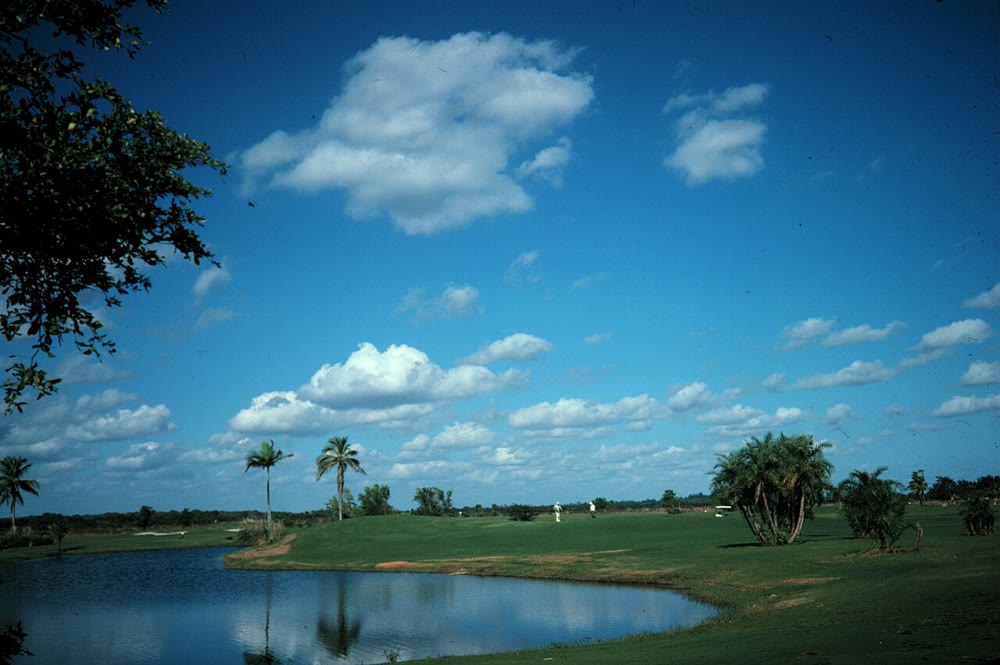
\includegraphics[height=4.5cm]{images/book2/g10-noaa-fair-weather-cumulus.jpg}\hspace{0.6em}%
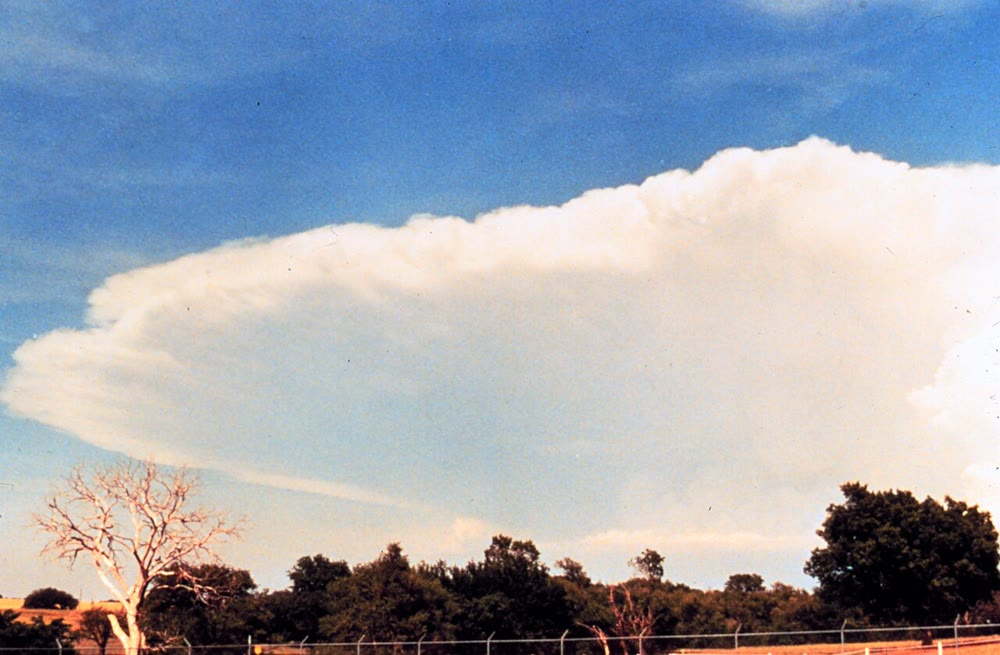
\includegraphics[height=4.5cm]{images/book2/g10-noaa-cumulonimbus-anvil.jpg}

{\small Kiri: kumulus cuaca cerah di atas Florida, dengan dasar datar pada
\omterm{def:g10:why-clouds-form:condensation-level}{aras kondensasinya}. Foto: Ralph F. Kresge, NOAA (domain publik). Kanan:
puncak berbentuk landasan tempa sebuah kumulonimbus pada tahap awal badai.
Foto: NOAA National Severe Storms Laboratory (domain publik).}
\end{omfigure}

\section{Empat cara mengangkat udara}

Udara naik karena empat sebab.
\begin{itemize}
  \item \textbf{Pemanasan dari bawah.} Pada hari yang cerah, tanah
        menghangatkan udara di atasnya; gelembung-gelembung udara hangat naik
        dari bagian tanah yang paling panas. Gelembung-gelembung inilah yang
        menghasilkan kumulus sore hari.
  \item \textbf{Pegunungan.} Angin yang bertiup ke arah pegunungan dipaksa
        naik menyusuri lerengnya.
  \item \textbf{Front.} Di tempat massa udara hangat dan dingin bertemu, udara
        hangat yang lebih ringan naik di atas udara dingin, atau udara dingin
        menyusup ke bawahnya (Buku 1, kelas 8).
  \item \textbf{Konvergensi.} Bila angin-angin mengalir menyatu di dekat
        tanah, udara tidak punya jalan lain selain ke atas, seperti pada sabuk
        udara naik di dekat khatulistiwa dan di pusat depresi.
\end{itemize}

\begin{method}[Mengikuti parsel melewati gunung]\label{met:g10:why-clouds-form:mountain}
\begin{enumerate}
  \item Tentukan \omterm{def:g10:why-clouds-form:condensation-level}{aras kondensasi} dengan aturan 125 meter; sampai aras itu
        parsel mendingin \qty{9.8}{\degreeCelsius/km}.
  \item Dari sana sampai ke puncak, parsel mendingin dengan laju \omterm{def:g10:why-clouds-form:humidity}{jenuh}; air
        yang mengembun jatuh sebagai hujan atau salju di lereng di hadapan
        angin.
  \item Di balik puncak parsel turun dalam keadaan tak \omterm{def:g10:why-clouds-form:humidity}{jenuh}: parsel
        menghangat \qty{9.8}{\degreeCelsius/km} sepanjang jalan turun.
\end{enumerate}
\end{method}

\begin{example}[Angin hangat kering di lereng di balik angin]\label{ex:g10:why-clouds-form:lee}
% ledger: iapws:vapour-pressure, nist:water-latent (all values computed in figdata/grade-10/clouds.py)
Udara di permukaan laut bersuhu \qty{20}{\degreeCelsius}, dengan \omterm{def:g10:why-clouds-form:dew-point}{titik embun}
\qty{12}{\degreeCelsius}, didorong melewati punggung pegunungan setinggi
\qty{2500}{m}. Udara itu menjadi \omterm{def:g10:why-clouds-form:humidity}{jenuh} pada $125 \times 8 = \qty{1000}{m}$,
pada sekitar \qty{10}{\degreeCelsius}. Dari sana sampai ke puncak, udara itu
mendingin dengan laju \omterm{def:g10:why-clouds-form:humidity}{jenuh} menjadi sekitar \qty{2}{\degreeCelsius}, dan
kehilangan sekitar sepertiga airnya sebagai hujan (dari \num{8.7} menjadi
\qty{6.0}{g/kg}). Ketika menuruni sisi seberang, udara itu menghangat dengan
laju kering sepanjang \qty{2.5}{km}: udara itu mencapai dataran pada sekitar
\qty{27}{\degreeCelsius}, tujuh derajat lebih hangat daripada saat berangkat,
dengan \omterm{def:g10:why-clouds-form:humidity}{kelembapan relatif} sekitar \qty{27}{\percent}. Angin hangat dan kering
seperti itu bertiup di lereng di balik angin banyak pegunungan.
\end{example}

\begin{omfigure}
\begin{tikzpicture}[font=\footnotesize, >={Stealth[length=2mm]}]
  \fill[omExo!30] (0,0) -- (3.5,0.3) -- (6,3.0) -- (8.5,0.3) -- (12,0) -- (12,-0.25) -- (0,-0.25) -- cycle;
  \draw[thick, black!70] (0,0) -- (3.5,0.3) -- (6,3.0) -- (8.5,0.3) -- (12,0);
  \draw[black!40, dashed] (0,1.2) -- (4.6,1.2);
  \node[anchor=south west, black!60, align=left] at (0.1,1.22) {aras\\kondensasi, \qty{1000}{m}};
  \foreach \x in {3.62,3.86,4.1} \draw[omDef!60] (\x,1.2) -- (\x-0.06,{0.3+(\x-0.06-3.5)*1.08+0.04});
  \pic[scale=1.1, transform shape] at (4.6,1.22) {puffycloud};
  \pic[scale=0.9, transform shape] at (5.0,2.2) {puffycloud};
  \draw[->, thick, omDef!80!black] (0.2,0.25) -- (2.8,0.5) .. controls (3.6,0.75) .. (4.4,1.7) -- (5.4,2.9) .. controls (5.8,3.4) and (6.2,3.4) .. (6.6,2.9) -- (7.6,1.7) .. controls (8.4,0.75) .. (9.2,0.5) -- (11.8,0.25);
  \node[anchor=east, align=right] at (3.4,2.15) {\qty{10}{\degreeCelsius}, jenuh};
  \node[anchor=south, align=center] at (6.0,3.45) {puncak \qty{2500}{m}: \qty{2}{\degreeCelsius}};
  \node[anchor=west, align=left] at (7.75,2.1) {turun dan menghangat\\\qty{9.8}{\degreeCelsius/km}};
  \node[anchor=north, align=center] at (1.0,-0.3) {\qty{20}{\degreeCelsius}\\titik embun \qty{12}{\degreeCelsius}};
  \node[anchor=north, align=center] at (11.0,-0.3) {\qty{27}{\degreeCelsius}\\titik embun \qty{6}{\degreeCelsius}};
  \node[anchor=north, black!60] at (4.0,-0.3) {hadapan angin: hujan};
  \node[anchor=north, black!60] at (8.2,-0.3) {balik angin: kering};
\end{tikzpicture}

{\small Parsel udara yang melintasi punggung pegunungan (suhu dihitung; skala
tegak dibesar-besarkan). Parsel mendingin dengan laju kering sampai \omterm{def:g10:why-clouds-form:condensation-level}{aras
kondensasinya}, dengan laju \omterm{def:g10:why-clouds-form:humidity}{jenuh} yang lebih lambat di atasnya sambil
kehilangan air sebagai hujan, lalu menghangat dengan laju kering sepanjang
jalan turun di lereng di balik angin.}
\end{omfigure}

\section{Dari titik-titik air menjadi hujan dan salju}

Uap air tidak mudah mengembun di udara yang benar-benar bersih. Titik-titik
air terbentuk pada butir-butir materi.

\begin{definition}[Inti kondensasi]\label{def:g10:why-clouds-form:nucleus}
Yang disebut \emph{inti kondensasi}\index{inti kondensasi} adalah partikel
sangat kecil yang melayang di udara --- sebutir garam laut, debu, asap, atau
jelaga --- tempat uap air mengembun membentuk titik awan.
\end{definition}

\omterm{def:g10:why-clouds-form:nucleus}{Inti kondensasi} yang khas berukuran sekitar \qty{0.0002}{mm}, titik awan
sekitar \qty{0.02}{mm}, tetes gerimis \qty{0.5}{mm}, dan tetes hujan sekitar
\qty{2}{mm}. Tetes hujan seratus kali lebih lebar daripada titik awan, jadi
volumenya $100^3$ kali lebih besar: sejuta titik awan membentuk satu tetes
hujan. Titik awan begitu kecil sehingga arus udara naik yang paling lemah pun
membuatnya tetap melayang; agar hujan dapat jatuh, titik-titik air harus
tumbuh seratus kali lipat.
% ledger: jpl:drop-sizes

\begin{omfigure}
\begin{tikzpicture}
\begin{axis}[width=0.9\linewidth, height=3.4cm, xmode=log, xmin=1e-4, xmax=10,
  ymin=0, ymax=1, axis y line=none, axis x line*=bottom,
  xlabel={diameter (mm), skala logaritmik}, tick label style={font=\small},
  label style={font=\small}, clip=false]
\addplot[only marks, mark=*, omDef!85!black, mark size=2.5pt] coordinates {(0.0002,0.3) (0.02,0.3) (0.5,0.3) (2,0.3)};
\node[anchor=south, font=\footnotesize, align=center] at (axis cs:0.0002,0.42) {inti\\kondensasi};
\node[anchor=south, font=\footnotesize, align=center] at (axis cs:0.02,0.42) {titik\\awan};
\node[anchor=south, font=\footnotesize, align=center] at (axis cs:0.5,0.42) {gerimis};
\node[anchor=south, font=\footnotesize, align=center] at (axis cs:2,0.42) {tetes hujan};
\end{axis}
\end{tikzpicture}

{\small Ukuran-ukuran khas, pada skala yang setiap langkahnya sepuluh kali
langkah sebelumnya: setiap benda sekitar seratus kali lebih lebar daripada
benda sebelumnya, kecuali gerimis. Data: NASA Jet Propulsion Laboratory.}
\end{omfigure}

Ada dua proses yang membuatnya tumbuh.

\begin{definition}[Proses hujan hangat; proses kristal es]\label{def:g10:why-clouds-form:rain-processes}
Dalam \emph{proses hujan hangat}\index{proses hujan hangat}, titik-titik air
yang lebih besar di dalam awan jatuh lebih cepat daripada yang kecil,
bertumbukan dengannya, dan bergabung, sehingga makin besar selama jatuh.
Dalam \emph{proses kristal es}\index{proses kristal es}, di bagian awan yang
lebih dingin daripada \qty{0}{\degreeCelsius} tempat kristal es dan
titik-titik air superdingin (cair di bawah \qty{0}{\degreeCelsius})
bercampur, kristal-kristal itu tumbuh dengan mengambil uap yang diuapkan
titik-titik air; kristal itu jatuh sebagai kepingan salju, dan mencair
menjadi tetes hujan jika udara di bawahnya hangat.
\end{definition}

\omterm{def:g10:why-clouds-form:rain-processes}{Proses kristal es} bekerja karena kandungan \omterm{def:g10:why-clouds-form:humidity}{jenuh} di atas es lebih rendah
daripada di atas air cair pada suhu yang sama: pada
\qty{-10}{\degreeCelsius} tekanan uap \omterm{def:g10:why-clouds-form:humidity}{jenuh} adalah \qty{287}{Pa} di atas air
dan \qty{260}{Pa} di atas es. Udara yang \omterm{def:g10:why-clouds-form:humidity}{jenuh} bagi titik-titik air
mengandung uap \qty{10}{\percent} lebih banyak daripada yang dapat ditanggung
es: uap mengembun pada kristal, dan titik-titik air menguap untuk
menggantikannya.
% ledger: iapws:vapour-pressure, iapws:melt-subl (computed in figdata/grade-10/clouds.py)

\begin{remark}[Kalor laten memberi makan badai]\label{rem:g10:why-clouds-form:latent}
Setiap kilogram air yang mengembun di dalam awan memberikan sekitar
\qty{2.5}{MJ} kepada udara, yaitu \omterm{def:g10:earth-energy-budget:latent-heat}{kalor laten} yang diambil dari laut atau dari
tanah ketika air itu menguap (\cref{ch:g10:earth-energy-budget}). Kalor inilah
yang membuat laju \omterm{def:g10:why-clouds-form:humidity}{jenuh} lebih lambat daripada laju kering dan membuat
kumulonimbus terus naik; \cref{ch:g10:storms-and-cyclones} mengikutinya sampai
ke badai-badai terbesar.
\end{remark}
% ledger: nist:water-latent

\section{Latihan}

Untuk latihan-latihan ini, gunakan kandungan \omterm{def:g10:why-clouds-form:humidity}{jenuh} (dalam \unit{g/kg}, pada
tekanan permukaan laut) pada tabel di bawah, laju kering
\qty{9.8}{\degreeCelsius/km}, penurunan \omterm{def:g10:why-clouds-form:dew-point}{titik embun}
\qty{1.8}{\degreeCelsius/km}, dan laju \omterm{def:g10:why-clouds-form:humidity}{jenuh} \qty{5}{\degreeCelsius/km}.
% ledger: iapws:vapour-pressure (table from figdata/out/grade-10-clouds-sat.dat, rounded)

\begin{center}
\small
\begin{tabular}{l*{11}{c}}
\hline
suhu (\unit{\degreeCelsius}) & 0 & 4 & 8 & 10 & 12 & 14 & 16 & 20 & 24 & 28 & 30 \\
kandungan \omterm{def:g10:why-clouds-form:humidity}{jenuh} (\unit{g/kg}) & 3.8 & 5.0 & 6.7 & 7.6 & 8.7 & 10.0 & 11.4 & 14.7 & 18.9 & 24.1 & 27.2 \\
\hline
\end{tabular}
\end{center}

\begin{exercise}[$\star$]\label{exo:g10:why-clouds-form:1}
Definisikan \omterm{def:g10:why-clouds-form:humidity}{kelembapan relatif} dan \omterm{def:g10:why-clouds-form:dew-point}{titik embun} udara.
\end{exercise}

\begin{exercise}[$\star$]\label{exo:g10:why-clouds-form:2}
Dari tabel, sebutkan kandungan \omterm{def:g10:why-clouds-form:humidity}{jenuh} pada \num{0}, \num{10},
\num{20}, dan \qty{30}{\degreeCelsius}. Kira-kira dengan faktor berapa
kandungan itu bertambah untuk setiap pemanasan \qty{10}{\degreeCelsius}?
\end{exercise}

\begin{exercise}[$\star$]\label{exo:g10:why-clouds-form:3}
Udara bersuhu \qty{24}{\degreeCelsius} mengandung \qty{10.0}{g/kg} uap air.
Tentukan \omterm{def:g10:why-clouds-form:humidity}{kelembapan relatif} dan \omterm{def:g10:why-clouds-form:dew-point}{titik embunnya}.
\end{exercise}

\begin{exercise}[$\star$]\label{exo:g10:why-clouds-form:4}
Jelaskan mengapa segelas air es ``berkeringat'' pada musim panas, dan mengapa
hal itu tidak terjadi di dalam ruangan pada hari musim dingin yang sangat
kering.
\end{exercise}

\begin{exercise}[$\star$]\label{exo:g10:why-clouds-form:5}
Sebutkan empat cara udara dibuat naik, beserta satu contoh untuk masing-masing.
\end{exercise}

\begin{exercise}[$\star\star$]\label{exo:g10:why-clouds-form:6}
Dengan \cref{prop:g10:why-clouds-form:lcl}, tentukan ketinggian dasar awan
untuk udara bersuhu \qty{30}{\degreeCelsius} dengan \omterm{def:g10:why-clouds-form:dew-point}{titik embun}
\qty{18}{\degreeCelsius}, dan untuk udara bersuhu \qty{22}{\degreeCelsius}
dengan \omterm{def:g10:why-clouds-form:dew-point}{titik embun} \qty{20}{\degreeCelsius}. Hari manakah yang kemungkinan
kelabu dengan awan rendah?
\end{exercise}

\begin{exercise}[$\star\star$]\label{exo:g10:why-clouds-form:7}
Sebuah parsel udara tak \omterm{def:g10:why-clouds-form:humidity}{jenuh} meninggalkan tanah pada
\qty{18}{\degreeCelsius}. Berapa suhunya pada ketinggian \qty{1}{km} dan
\qty{2}{km}, jika parsel itu tetap tak \omterm{def:g10:why-clouds-form:humidity}{jenuh}? Bila turun kembali dari
\qty{2}{km}, pada suhu berapa parsel itu mencapai tanah?
\end{exercise}

\begin{exercise}[$\star\star$]\label{exo:g10:why-clouds-form:8}
Pengukuran balon sonde menunjukkan suhu turun \qty{4}{\degreeCelsius} per km.
Apakah udara itu \omterm{def:g10:why-clouds-form:stability}{stabil} bagi parsel tak \omterm{def:g10:why-clouds-form:humidity}{jenuh}? Bagi parsel \omterm{def:g10:why-clouds-form:humidity}{jenuh}? Pada sore
hari yang panas, suhu turun \qty{12}{\degreeCelsius} pada kilometer pertama di
atas tanah: apa yang terjadi pada gelembung-gelembung udara hangat?
\end{exercise}

\begin{exercise}[$\star\star$]\label{exo:g10:why-clouds-form:9}
Udara \omterm{def:g10:why-clouds-form:humidity}{jenuh} bersuhu \qty{20}{\degreeCelsius} didinginkan menjadi
\qty{10}{\degreeCelsius}. Berapa gram air yang mengembun per kilogram udara?
Ke mana perginya \omterm{def:g10:earth-energy-budget:latent-heat}{kalor laten} yang dilepaskan?
\end{exercise}

\begin{exercise}[$\star\star$]\label{exo:g10:why-clouds-form:10}
Berapa titik awan berdiameter \qty{0.02}{mm} yang membentuk satu tetes gerimis
berdiameter \qty{0.5}{mm}? Satu tetes hujan berdiameter \qty{2}{mm}?
\end{exercise}

\begin{exercise}[$\star\star$]\label{exo:g10:why-clouds-form:11}
Jelaskan, langkah demi langkah, mengapa pada waktu fajar setelah malam yang
cerah dan tenang kabut terbentuk di lembah, bukan di puncak bukit.
\end{exercise}

\begin{exercise}[$\star\star\star$]\label{exo:g10:why-clouds-form:12}
Laju kering adalah $a$ dan \omterm{def:g10:why-clouds-form:dew-point}{titik embun} turun dengan laju $b$ (keduanya dalam
\unit{\degreeCelsius/km}). Tunjukkan bahwa \omterm{def:g10:why-clouds-form:condensation-level}{aras kondensasi} berada pada
$z = (T - T_d)/(a - b)$. Di atas sebuah dataran tinggi \omterm{def:g10:why-clouds-form:dew-point}{titik embun} turun
\qty{1.7}{\degreeCelsius/km}: menjadi apakah aturan ``\qty{125}{m} per
derajat''?
\end{exercise}

\begin{exercise}[$\star\star\star$]\label{exo:g10:why-clouds-form:13}
Udara di permukaan laut bersuhu \qty{15}{\degreeCelsius}, dengan \omterm{def:g10:why-clouds-form:dew-point}{titik embun}
\qty{11}{\degreeCelsius}, melintasi punggung pegunungan setinggi
\qty{2000}{m}. Dengan mengikuti \cref{met:g10:why-clouds-form:mountain},
tentukan \omterm{def:g10:why-clouds-form:condensation-level}{aras kondensasi}, suhu di sana, suhu di puncak, dan suhu udara itu
ketika mencapai dataran di sisi seberang.
\end{exercise}

\begin{exercise}[$\star\star\star$]\label{exo:g10:why-clouds-form:14}
Pada \qty{-20}{\degreeCelsius} tekanan uap \omterm{def:g10:why-clouds-form:humidity}{jenuh} adalah \qty{126}{Pa} di atas
air dan \qty{103}{Pa} di atas es. Berapa persen udara yang \omterm{def:g10:why-clouds-form:humidity}{jenuh} bagi
titik-titik air itu lewat \omterm{def:g10:why-clouds-form:humidity}{jenuh} bagi es? Bandingkan dengan
\qty{-10}{\degreeCelsius}, dan sebutkan di bagian awan mana \omterm{def:g10:why-clouds-form:rain-processes}{proses kristal es}
bekerja paling baik.
\end{exercise}

\begin{exercise}[$\star\star\star$]\label{exo:g10:why-clouds-form:15}
Udara di sekitarnya mendingin \qty{6.5}{\degreeCelsius/km}. Sebuah parsel
mula-mula bersuhu sama dengan sekitarnya dan naik \qty{1}{km}. Hitung selisih
suhunya dengan suhu udara di sekitarnya jika parsel itu tak \omterm{def:g10:why-clouds-form:humidity}{jenuh}, lalu jika
parsel itu \omterm{def:g10:why-clouds-form:humidity}{jenuh}. Jelaskan ungkapan ``\omterm{def:g10:why-clouds-form:stability}{tidak stabil} bersyarat''.
\end{exercise}

\section{Soal: Suatu Sore Musim Panas di Atas Dataran}

\begin{problem}[{Soal akhir pekan --- dari kelembapan pagi hari sampai dasar
awan sore hari}]
\label{pb:g10:why-clouds-form:1}
% ledger: iapws:vapour-pressure, nist:water-latent (all results computed in figdata/grade-10/clouds.py or from the rounded data below; the sounding is sounding A, invented)
Di atas sebuah dataran yang luas, pada suatu hari musim panas, udara di dekat
tanah mengandung \qty{11.4}{g/kg} uap air sepanjang hari. Suhunya
\qty{20}{\degreeCelsius} pada pagi hari dan \qty{28}{\degreeCelsius} pada sore
hari. Pengukuran balon sonde (contoh rekaan) memberikan suhu udara di atasnya:

\begin{center}
\small
\begin{tabular}{l*{8}{c}}
\hline
ketinggian (km) & 0 & 0.5 & 1.0 & 1.5 & 2.5 & 3.5 & 3.6 & 4.0 \\
suhu (\unit{\degreeCelsius}) & 28.0 & 23.1 & 18.2 & 13.4 & 6.9 & 0.4 & $-0.3$ & 1.2 \\
\hline
\end{tabular}
\end{center}

\noindent Gunakan tabel kandungan \omterm{def:g10:why-clouds-form:humidity}{jenuh} dan laju-laju yang diberikan sebelum
latihan.

\medskip
\noindent\textbf{Bagian I --- Kelembapan.}
\begin{enumerate}
  \item Sebutkan kandungan \omterm{def:g10:why-clouds-form:humidity}{jenuh} pada \qty{20}{\degreeCelsius}.
  \item Hitung \omterm{def:g10:why-clouds-form:humidity}{kelembapan relatif} pada pagi hari.
  \item Tentukan \omterm{def:g10:why-clouds-form:dew-point}{titik embun} udara itu.
  \item Hitung \omterm{def:g10:why-clouds-form:humidity}{kelembapan relatif} pada sore hari.
  \item Apakah udara menjadi lebih kering pada sore hari? Jelaskan.
\end{enumerate}

\medskip
\noindent\textbf{Bagian II --- Malam dan embun.}
\begin{enumerate}[resume]
  \item Pada malam hari udara di dekat tanah mendingin. Pada suhu berapa
        embun mulai terbentuk?
  \item Jika udara mendingin menjadi \qty{12}{\degreeCelsius}, berapa gram
        air per kilogram udara yang telah mengembun?
  \item Mengapa embun terbentuk pada rumput dan atap mobil sebelum terbentuk
        di udara?
\end{enumerate}

\medskip
\noindent\textbf{Bagian III --- Hasil sonde.}
\begin{enumerate}[resume]
  \item Hitung laju penurunan suhu antara \num{0} dan \qty{1.5}{km}.
        Bandingkan dengan laju kering.
  \item Hitung laju itu antara \num{1.5} dan \qty{3.5}{km}.
  \item Apakah udara antara \num{1.5} dan \qty{3.5}{km} \omterm{def:g10:why-clouds-form:stability}{stabil} bagi parsel
        tak \omterm{def:g10:why-clouds-form:humidity}{jenuh}? Bagi parsel \omterm{def:g10:why-clouds-form:humidity}{jenuh}?
  \item Apa yang terjadi antara \num{3.6} dan \qty{4.0}{km}? Apa akibatnya
        bagi awan yang sedang tumbuh ke atas?
\end{enumerate}

\medskip
\noindent\textbf{Bagian IV --- Dasar awan.}
\begin{enumerate}[resume]
  \item Hitung selisih antara suhu udara dan \omterm{def:g10:why-clouds-form:dew-point}{titik embunnya} di tanah pada
        sore hari.
  \item Hitung suhu dan \omterm{def:g10:why-clouds-form:dew-point}{titik embun} sebuah gelembung udara ini setelah naik
        \qty{1}{km}, masih dalam keadaan tak \omterm{def:g10:why-clouds-form:humidity}{jenuh}.
  \item Berapa besar selisih keduanya telah menyusut? Dengan laju berapa
        selisih itu menyusut?
  \item Tunjukkan bahwa laju ini menghasilkan aturan ``\qty{125}{m} per
        derajat''.
  \item Berapa ketinggian dasar awan pada pagi hari?
  \item Jelaskan mengapa dasar kumulus naik sepanjang hari.
  \item Tuliskan persamaan yang menyatakan bahwa suhu gelembung sama dengan
        \omterm{def:g10:why-clouds-form:dew-point}{titik embunnya} pada ketinggian $z$ (dalam km).
  \item Selesaikan persamaan itu: pada ketinggian berapa dasar kumulus sore
        hari berada?
\end{enumerate}
\end{problem}
